\documentclass[10pt]{ltjsarticle}
\usepackage{layout,url}
\usepackage{graphicx}
\usepackage[haranoaji,deluxe]{luatexja-preset}
\usepackage{resume}
\pagestyle{empty}

\begin{document}
%\layout

\title{タイトル}

% 和文著者名
\author{
    著者その1 \thanks{所属その1}
    \and
    著者その2 \thanks{所属その2}
}

% 和文概要
\begin{abstract}
ここにアブストラクトを書く。そうです。
\end{abstract}

\maketitle
\thispagestyle{empty}

\section{はじめに}

%引用例\cite{example}を書いてみた.

\section{背景}

\subsection{hoge}
小見出し付きの文章.

\begin{enumerate}
\item 番号付き箇条書き 
\item 番号付き箇条書き
\end{enumerate}

\begin{itemize}
\item 箇条書き
\item 箇条書き
\end{itemize}

%---------------------------------------------

\section{研究目的}

\subsection{hoge}
画像を図\ref{sample}に示す。

\begin{figure}[htbp]
    \begin{center}
        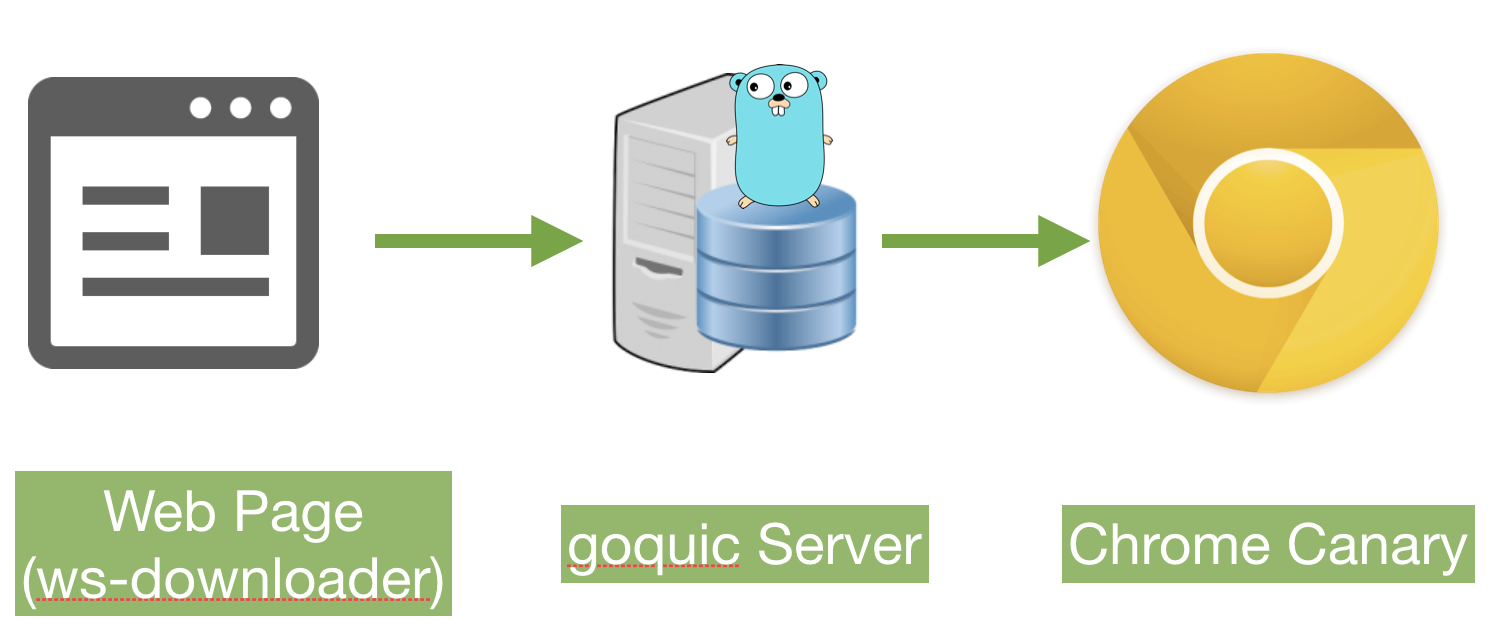
\includegraphics[width=6cm]{figure1.png}
        \caption{画像の例}
        \label{sample}
    \end{center}
\end{figure}
 
\subsection{fuga}
fugafuga

\section{関連研究}

\section{提案手法}

\section{評価}

\section{考察}

\bibliographystyle{junsrt}
\bibliography{resume}

\end{document}
% end of file
